\documentclass[11pt,a4paper]{article}

% --- PACKAGES ---
\usepackage[utf8]{inputenc}
\usepackage[margin=1in]{geometry}
\usepackage{amsmath, amsfonts, amssymb, amsthm}
\usepackage{xcolor}
\usepackage{tikz}
\usepackage[framemethod=tikz]{mdframed}
\usepackage{fancyhdr}
\usepackage{graphicx}
\usepackage{enumitem}
\usepackage{hyperref}

% Commands
\newcommand{\R}{\mathbb{R}}
\newcommand{\Q}{\mathbb{Q}}
\newcommand{\C}{\mathbb{C}}
\newcommand{\Z}{\mathbb{Z}}
\newcommand{\cl}[1]{\overline{#1}}

% --- COLOR PALETTE ---
\definecolor{primaryColor}{RGB}{28, 54, 115}      % Dark Navy (Definitions / Primary)
\definecolor{accentColor}{RGB}{0, 150, 136}        % Teal (Key Takeaways / Tips)
\definecolor{theoremColor}{RGB}{74, 20, 140}      % Deep Purple (Theorems / Propositions)
\definecolor{corollaryColor}{RGB}{21, 101, 192}    % Blue (Corollaries)
\definecolor{exampleColor}{RGB}{46, 125, 50}      % Forest Green (Examples)
\definecolor{cautionColor}{RGB}{198, 40, 40}      % Crimson Red (Cautions)
\definecolor{remarkColor}{RGB}{106, 27, 154}      % Amethyst (Remarks)
\definecolor{recallColor}{RGB}{41, 128, 185}      % Slate Blue (Recalls)
\definecolor{boxBg}{RGB}{245, 247, 250}          % Light Gray-Blue Background
\definecolor{exerciseColor}{RGB}{211, 84, 0}      % Rust/Orange (Exercises)

% --- PAGE SETUP (HEADERS & FOOTERS) ---
\setlength{\headheight}{14pt}
\renewcommand{\headrulewidth}{0.4pt}
% \renewcommand{\footrulewidth}{0.4pt}

% --- CUSTOM STYLED BOX TEMPLATE ---
\mdfdefinestyle{custombox}{
	backgroundcolor=boxBg,
	topline=false,
	rightline=false,
	bottomline=false,
	linewidth=2pt,
	innertopmargin=12pt,
	innerbottommargin=12pt,
	innerrightmargin=14pt,
	innerleftmargin=14pt,
	skipabove=12pt,
	skipbelow=12pt,
	splittopskip=20pt,
	splitbottomskip=12pt,
	nobreak=false
}

% Box Environment Declarations
\newmdenv[style=custombox, linecolor=primaryColor]{definitionbox}
\newmdenv[style=custombox, linecolor=accentColor]{tipbox}
\newmdenv[style=custombox, linecolor=theoremColor]{theorembox}
\newmdenv[style=custombox, linecolor=corollaryColor]{corollarybox}
\newmdenv[style=custombox, linecolor=theoremColor]{lemmabox}
\newmdenv[style=custombox, linecolor=exampleColor]{examplebox}
\newmdenv[style=custombox, linecolor=cautionColor]{cautionbox}
\newmdenv[style=custombox, linecolor=remarkColor]{remarkbox}
\newmdenv[style=custombox, linecolor=recallColor]{recallbox}
\newmdenv[style=custombox, linecolor=exerciseColor]{exercisebox}


% --- SHARED COUNTER FOR THEOREM-LIKE ENVIRONMENTS ---
\newcounter{thmcnt}[section]
\renewcommand{\thethmcnt}{\thesection.\arabic{thmcnt}}

% --- CUSTOM ENVIRONMENTS FOR BOXED SECTIONS ---
\newenvironment{definition}[1]{
	\begin{definitionbox}
		\textbf{\color{primaryColor}Definition (#1):} 
	}{
	\end{definitionbox}
}

\newenvironment{takeaway}{
	\begin{tipbox}
		\textbf{\color{accentColor}Key Takeaway:} 
	}{
	\end{tipbox}
}

\newenvironment{notation}[1]{
	\begin{definitionbox}
		\textbf{\color{primaryColor}Notation\ifx&#1&\else\ (#1)\fi:} 
	}{
	\end{definitionbox}
}

% --- CORRECTED CUSTOM ENVIRONMENTS ---

\newenvironment{theorem}[1][]{
	\def\temp{#1}%
	\refstepcounter{thmcnt}
	\begin{theorembox}
		\textbf{\color{theoremColor}Theorem \thethmcnt%
			\ifx\temp\empty\relax\else\ (#1)\fi:} 
	}{
	\end{theorembox}
}

\newenvironment{proposition}[1][]{
	\def\temp{#1}%
	\refstepcounter{thmcnt}
	\begin{theorembox}
		\textbf{\color{theoremColor}Proposition \thethmcnt%
			\ifx\temp\empty\relax\else\ (#1)\fi:} 
	}{
	\end{theorembox}
}

\newenvironment{corollary}[1][]{
	\def\temp{#1}%
	\refstepcounter{thmcnt}
	\begin{corollarybox}
		\textbf{\color{corollaryColor}Corollary \thethmcnt%
			\ifx\temp\empty\relax\else\ (#1)\fi:} 
	}{
	\end{corollarybox}
}

\newenvironment{lemma}[1][]{
	\def\temp{#1}%
	\refstepcounter{thmcnt}%
	\begin{lemmabox}
		\textbf{\color{theoremColor}Lemma \thethmcnt%
			\ifx\temp\empty\relax\else\ (#1)\fi:} 
	}{
	\end{lemmabox}
}

\newcounter{examplecnt}[section]
\newenvironment{example}[1][]{
	\stepcounter{examplecnt}
	\begin{examplebox}
		\textbf{\color{exampleColor}Example \arabic{examplecnt}\ifx&#1&\else\ (#1)\fi:} 
	}{
	\end{examplebox}
}

\newenvironment{caution}{
	\begin{cautionbox}
		\textbf{\color{cautionColor}Caution:} 
	}{
	\end{cautionbox}
}

\newenvironment{remark}{
	\begin{remarkbox}
		\textbf{\color{remarkColor}Remark:} 
	}{
	\end{remarkbox}
}

\newenvironment{recall}[1][]{
	\begin{recallbox}
		\textbf{\color{recallColor}Recall\ifx&#1&\else\ (#1)\fi:} 
	}{
	\end{recallbox}
}

% --- HYPERLINK SETUP ---
\hypersetup{
	colorlinks=true,
	linkcolor=primaryColor,
	urlcolor=accentColor,
	pageanchor=false
}

\newcounter{exercisecnt}[section]
\newenvironment{exercise}[1][]{
	\stepcounter{exercisecnt}
	\begin{exercisebox}
		\textbf{\color{exerciseColor}Exercise \arabic{exercisecnt}\ifx&#1&\else\ (#1)\fi:} 
	}{
	\end{exercisebox}
}

% --- CUSTOM LECTURE TITLE COMMAND ---
\newcommand{\lecturetitle}[2]{%
	\newpage
	\thispagestyle{plain} 
	\refstepcounter{section} 
	\phantomsection
	\addcontentsline{toc}{section}{Lecture #1: #2} 
	\vspace*{1em}
	\noindent\rule{\textwidth}{1.2pt} \\[-0.85\baselineskip]
	\noindent\rule{\textwidth}{0.4pt}
	\begin{center}
		\large \textsc{Lecture #1}
	\end{center}
	\begin{center}
		\Huge \textsc{#2}
	\end{center}
	\vspace{0.8em}
	\noindent\rule{\textwidth}{0.4pt} \\[-0.85\baselineskip]
	\noindent\rule{\textwidth}{1.2pt}
	\vspace{1.5em}
	\rhead{Lecture #1: #2}
}

\begin{document}
	
	% ==========================================
	% COVER PAGE WITH UNIVERSITY LOGO
	% ==========================================
	\begin{titlepage}
		\centering
		\thispagestyle{empty}
		
		% Cairo University Logo
		
\includegraphics[width=0.25\textwidth]{cairo_university_new_logo.png}\\[1em]
		
		% University / Department Header
		{\Large \textbf{Cairo University}}\\[0.3em]
		{\large \textsc{Department of Mathematics}}\\[2em]
		
		% Title & Subtitle
		{\Huge \textbf{Real Analysis}}\\[0.6em]
		{\Large \textbf{Lecture Notes}}\\[1.5em]
		
		% Central Figure: Hierarchy of Spaces
		\vfill
		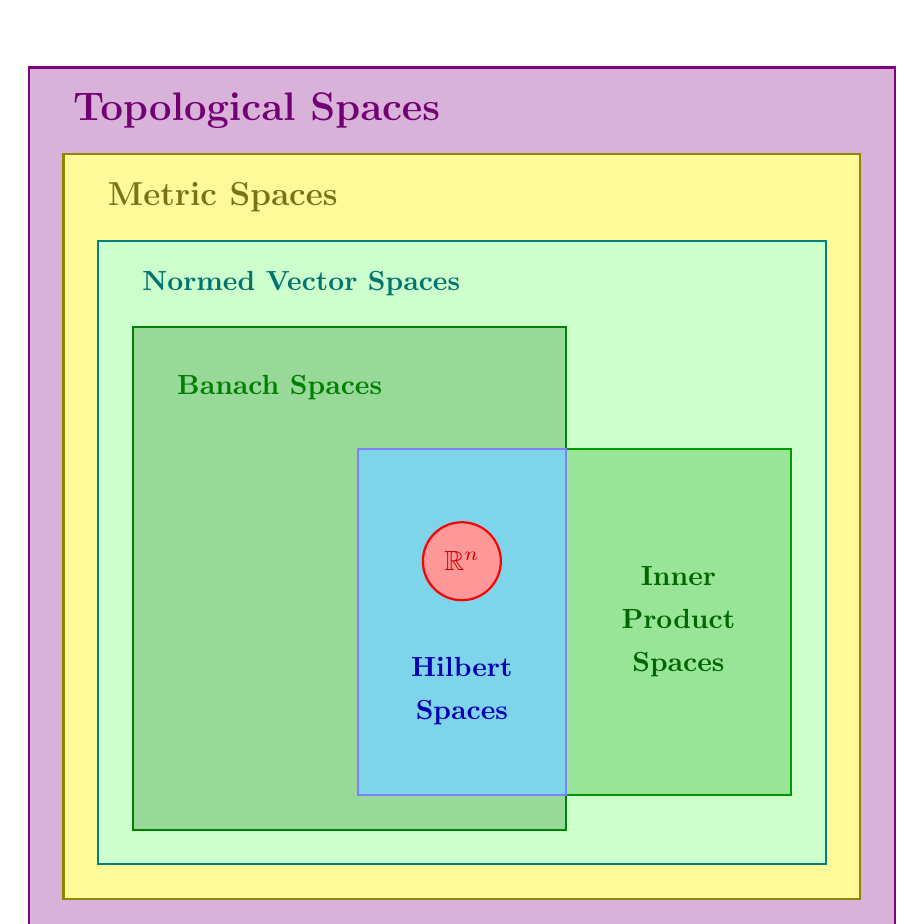
\begin{tikzpicture}[scale=1.1, font=\sffamily]
			
			% Topological Spaces
			\draw[fill=violet!30, draw=violet, thick] (0,0) rectangle (10,10);
			\node[text=violet!90!black, font=\bfseries\Large, anchor=west] at (0.4, 9.5) {Topological Spaces};
			
			% Metric Spaces
			\draw[fill=yellow!40, draw=olive, thick] (0.4, 0.4) rectangle (9.6, 9.0);
			\node[text=olive!80!black, font=\bfseries\large, anchor=west] at (0.8, 8.5) {Metric Spaces};
			
			% Normed Vector Spaces
			\draw[fill=green!20, draw=teal, thick] (0.8, 0.8) rectangle (9.2, 8.0);
			\node[text=teal!90!black, font=\bfseries, anchor=west] at (1.2, 7.5) {Normed Vector Spaces};
			
			% Banach Spaces
			\draw[fill=green!40!black, fill opacity=0.25, draw=green!50!black, thick] (1.2, 1.2) rectangle (6.2, 7.0);
			\node[text=green!50!black, font=\bfseries, anchor=west, opacity=1] at (1.6, 6.3) {Banach Spaces};
			
			% Inner Product Spaces 
			\draw[fill=green!60!black, fill opacity=0.25, draw=green!60!black, thick] (3.8, 1.6) rectangle (8.8, 5.6);
			\node[text=green!40!black, font=\bfseries, align=center, opacity=1] at (7.5, 3.6) {Inner\\[0.3em]Product\\[0.3em]Spaces};
			
			% Hilbert Spaces (Intersection of Banach and Inner Product)
			\draw[fill=cyan!50, draw=blue!50, thick, fill opacity=0.9] (3.8, 1.6) rectangle (6.2, 5.6);
			\node[text=blue!70!black, font=\bfseries, align=center] at (5.0, 2.8) {Hilbert\\[0.3em]Spaces};
			
			% R^n 
			\draw[fill=red!40, draw=red, thick, fill opacity=1] (5.0, 4.3) circle (0.45);
			\node[text=red!80!black, font=\bfseries] at (5.0, 4.3) {$\R^n$};
			
		\end{tikzpicture}
		\vfill
		
		% Author and Lecturer Details
		\vspace{1cm}
		\begin{minipage}{0.45\textwidth}
			\begin{flushleft}
				\textit{Written by:}\\
				\textbf{Mohamed Asubhi}
			\end{flushleft}
		\end{minipage}
		\begin{minipage}{0.45\textwidth}
			\begin{flushright}
				\textit{Lecturer:}\\
				\textbf{Prof. Mohamed Ramadan}
			\end{flushright}
		\end{minipage}\\[2.5em]
		
		% Date / Term
		{\large Fall Term 2026}
	\end{titlepage}
	
	\newpage
	
	% ==========================================
	% FRONT MATTER (ROMAN NUMERALS)
	% ==========================================
	\pagenumbering{roman} 
	\pagestyle{plain} 
	
	% ==========================================
	% TABLE OF CONTENTS
	% ==========================================
	\vspace*{1em}
	\noindent\rule{\textwidth}{1.2pt} \\[-0.85\baselineskip]
	\noindent\rule{\textwidth}{0.4pt}
	\begin{center}
		\huge \textsc{Contents}
	\end{center}
	\vspace{1.5em}
	
	\tableofcontents
	
	\newpage
	% ==========================================
	% ACKNOWLEDGMENTS (LARGER TEXT)
	% ==========================================
	\vspace*{1em}
	\noindent\rule{\textwidth}{1.2pt} \\[-0.85\baselineskip]
	\noindent\rule{\textwidth}{0.4pt}
	\begin{center}
		\huge \textsc{Acknowledgments}
	\end{center}
	\vspace{2em}
	
	{
		
		First and foremost, I would like to express my sincere gratitude to \textbf{Prof. Mohamed Ramadan}. These notes are based on his lectures, and I am deeply thankful for the foundational material he provided and his dedicated work with us.
		
		\vspace{1.5em}
		Special thanks to my friend \textbf{Mina Basilious} who helped very much in refining the text, and checked most of the proofs and material.
	}
	
	
	
	
	\newpage
	% ==========================================
	% MAIN CONTENT (ARABIC NUMERALS & FANCY HEADERS)
	% ==========================================
	\pagenumbering{arabic}
	\pagestyle{fancy}
	\fancyhf{}
	\lhead{\textbf{M331: Real Analysis}}
	% \rhead{\leftmark}
	% \lfoot{\textit{Dept. of Math, Cairo University}}
	\cfoot{\thepage}
	
	
	\lecturetitle{1}{Introduction to Metric Spaces}
	% \textit{Date: Sep 26, 2026}
	
	\subsection{Metric Space}
	\begin{definition}{Metric Space}By Metric Spaces $(M,d)$ we mean a non-empty set $M$ with function 
		\[
		d: M \times M \to \R
		\]
		such that:
		\begin{enumerate}
			\item \textbf{Non-negativity and Definiteness:}
			\[
			d(x,y)\geq 0, \quad \forall x,y \in M
			\]
			and
			\[
			d(x,y) = 0 \iff x=y
			\]
			
			\item \textbf{Symmetry:}
			\[
			d(x,y)=  d(y,x), \quad \forall x,y \in M
			\]
			
			\item \textbf{Triangle Inequality:}
			\[
			d(x,z)\leq d(x,y)+d(y,z), \quad \forall x,y,z \in M
			\]
		\end{enumerate}
	\end{definition}
	
	\begin{example}Let $M = \mathbb{R}$ and define the distance function as:
		\[ d(x, y) = |x - y| \]
		To show it is a metric, we verify the three main properties:
		\begin{enumerate}
			\item \textbf{Non-negativity:} 
			\[d(x, y) = |x - y| \geq 0\]
			and if $d(x, y) = 0$, then $|x - y| = 0 \implies x = y$.
			\item \textbf{Symmetry:}
			\[d(x, y) = |x - y| = |-(y - x)| = |y - x| = d(y, x)\]
			\item \textbf{Triangle Inequality:} 
			\[ d(x, z) = |x - z| = |(x - y) + (y - z)| \leq |x - y| + |y - z| = d(x, y) + d(y, z) \]
		\end{enumerate}
		For any two complex numbers $z_1 = x_1 + iy_1$ and $z_2 = x_2 + iy_2$, the distance (Euclidean metric) is defined as:
		\[ |z_1 - z_2| = \sqrt{(x_1 - x_2)^2 + (y_1 - y_2)^2} \]
	\end{example}
	
	\begin{example}Let $M$ be any non-empty set and define the distance function as:
		\[ d(x, y) = \begin{cases} 0 & \text{if } x = y \\ 1 & \text{if } x \neq y \end{cases} \]
		
		This satisfies:
		\begin{enumerate}
			\item \textbf{Non-negativity:} it is clear that $d(x,y) \ge 0$. And, if $d(x,y) = 0$, then $x = y$ by the definition of the metric $d$.
			\item \textbf{Symmetry:} it is clear that $d(x,y) = d(y,x)$.
			\item \textbf{Triangle Inequality:} We want to show that $d(x, z) \leq d(x, y) + d(y, z)$ for any $x, y, z \in M$. We consider two cases:
			\begin{itemize}
				\item \textbf{Case 1 ($x = z$):} Then $d(x, z) = 0$. Since distances are non-negative ($d(x, y) \geq 0$ and $d(y, z) \geq 0$), their sum is $\geq 0$, so $0 \leq d(x, y) + d(y, z)$ holds.
				\item \textbf{Case 2 ($x \neq z$):} Then $d(x, z) = 1$. Since $x \neq z$, the point $y$ cannot be equal to both $x$ and $z$ simultaneously. Thus, at least one of $d(x, y)$ or $d(y, z)$ must equal $1$, meaning $d(x, y) + d(y, z) \geq 1$. Therefore, $1 \leq d(x, y) + d(y, z)$ holds.
			\end{itemize}
		\end{enumerate}
	\end{example}
	
	
	\begin{example}On $\R^2$, for points $x = (x_1, x_2)$ and $y = (y_1, y_2)$, we may define different metrics:
		\begin{enumerate}
			\item \[ d_1(x, y) = |x_1 - y_1| + |x_2 - y_2| \]
			\item \[ d_2(x, y) = \sqrt{(x_1 - y_1)^2 + (x_2 - y_2)^2} \]
			\item \[ d_\infty(x, y) = \max(|x_1 - y_1|, |x_2 - y_2|) \]
			\item \[ d_p(x, y) = \left( |x_1 - y_1|^p + |x_2 - y_2|^p \right)^{1/p}, \quad p \ge 1 \]
		\end{enumerate}
	\end{example}
	
	
	\subsection{Cauchy--Schwarz Inequality}
	\begin{theorem}[Cauchy--Schwarz Inequality]
		For any  $(a_1, a_2, \dots, a_n)$ and $(b_1, b_2, \dots, b_n)$ in $\mathbb{R}^n$, the Cauchy--Schwarz inequality states:
		\[ \left( \sum_{i=1}^{n} a_i b_i \right)^2 \leq \left( \sum_{i=1}^{n} a_i^2 \right) \left( \sum_{i=1}^{n} b_i^2 \right) \]
	\end{theorem}
	
	\begin{proof}
		Consider the non-negative quadratic expression for any real parameter $t$:
		\[ \sum_{i=1}^{n} (a_i - t b_i)^2 \geq 0 \]
		
		\noindent Expanding this gives:
		\[ \sum_{i=1}^{n} \left(a_i^2 - 2t a_i b_i + t^2 b_i^2\right) = \left(\sum_{i=1}^{n} a_i^2\right) - 2t \left(\sum_{i=1}^{n} a_i b_i\right) + t^2 \left(\sum_{i=1}^{n} b_i^2\right) \geq 0 \]
		
		\noindent Letting $A = \sum_{i=1}^{n} a_i^2$, $B = \sum_{i=1}^{n} a_i b_i$, and $C = \sum_{i=1}^{n} b_i^2$, the inequality becomes a quadratic in $t$:
		\[ A - 2Bt + Ct^2 \geq 0 \]
		
		\noindent Assume first that $C > 0$. For the quadratic $Ct^2 - 2Bt + A$ to remain non-negative for all real $t$, its discriminant $\Delta = (-2B)^2 - 4AC$ must be less than or equal to zero:
		\[ 4B^2 - 4AC \leq 0 \implies B^2 \leq AC \]
		
		\noindent Substituting back $A$, $B$, and $C$ yields the Cauchy--Schwarz inequality:
		\[ \left( \sum_{i=1}^{n} a_i b_i \right)^2 \leq \left( \sum_{i=1}^{n} a_i^2 \right) \left( \sum_{i=1}^{n} b_i^2 \right) \]
		
		\noindent Note, however, that this proof is valid only if $C = \sum_{i=1}^{n} b_i^2 > 0$. If $C = 0$, then all $b_i = 0$, and the inequality holds trivially since both sides equal zero.
	\end{proof}
	
	\lecturetitle{2}{Open Balls and Metric Space Topology}
	% \textit{Date: Sep 29, 2026}
	
	\subsection{Open Balls and Bounded Sets}
	
	\begin{definition}{Open Ball}Let $(M,d)$ be a metric space, $x_0 \in M$ and $r \in \mathbb{R}^{+}$. The set defined by 
		\[
		B(x_0; r) := \{x \in M : d(x_0, x) < r\}
		\]
		is called the open ball centered at $x_0$ with radius $r$.
	\end{definition}
	
	\begin{remark}Boundedness in $\mathbb{R}$:
		A subset $E \subseteq \mathbb{R}$ is bounded if and only if any of the following equivalent conditions hold:
		\begin{enumerate}
			\item There exist real numbers $l, L \in \mathbb{R}$ such that:
			\[
			l < x < L \quad \forall x \in E
			\]
			\item There exists a positive real number $M > 0$ such that:
			\[
			-M < x < M \quad (\text{or } |x| < M) \quad \forall x \in E
			\]
		\end{enumerate}
	\end{remark}
	
	\begin{definition}{Bounded Set}A subset $E$ of a metric space $(M,d)$ is called bounded if it is contained in a ball $E \subseteq B(x_0; r)$ for some $x_0 \in M$ and $r \in \mathbb{R}^{+}$.
	\end{definition}
	
	\begin{theorem}
		The union of any two (finite number of) bounded set is bounded
	\end{theorem}
	\begin{proof}
		Let $E_1$ and $E_2$ be bounded sets, that is, $\exists x_1, x_2 \in M;~ r_1,r_2\in\R^+$ with
		\[
		E_k \subseteq B(x_k;r_k), \quad k=1,2
		\]
		
		\noindent It suffices to find one open ball containing both of these balls. Let:
		\[
		R = \max \{ d(x_1, x_2) + r_2 , r_1 \}
		\]
		Then $B(x_1; r_1) \cup B(x_2; r_2) \subseteq B(x_1; R)$. \medskip
		
		\noindent For if $x \in B(x_1; r_1)$, then $d(x_1, x) < r_1 \le R$. If $x \in B(x_2; r_2)$, then $d(x_2, x) < r_2$, and by the triangle inequality
		\[
		d(x_1, x) \le d(x_1, x_2) + d(x_2, x) < d(x_1, x_2) + r_2 \le R.
		\]
		
		\noindent So in both cases $x \in B(x_1; R)$. Hence $E_1 \cup E_2 \subseteq B(x_1; R)$, and the union is bounded.
	\end{proof}
	
	\subsection{Interior Points and Open Sets}
	
	\begin{definition}{Interior Point}Let $E \subseteq M$ where $(M,d)$ is a metric space. A point $x_0 \in E$ is called an interior point of $E$ if there is $\varepsilon > 0$ such that $B(x_0; \varepsilon) \subseteq E$. The set of all interior points of $E$ is denoted by $E^\circ$.
	\end{definition}
	
	\begin{definition}{Open Set}A subset $G$ of a metric space $(M,d)$ is called an open set if all its points are interior points, that is, $G = G^\circ$.
	\end{definition}
	
	
	\begin{definition}{Intervals}$I \subseteq \R $ is called an interval if 
		\[
		\forall x,y,z \in  \R, \quad x < y < z, \quad x,z \in I \implies y \in I
		\]
	\end{definition} 
	
	\begin{example}\begin{itemize}
			\item Let $G = \left]0,1\right[ \implies G^\circ = G$.
			\item Let $E = [a, b]$. Then $E^\circ = (a, b)$.
		\end{itemize}
	\end{example}
	
	
	
	
	\begin{example}In $\mathbb{R}^2$ (with the Euclidean distance), let $E = [0,1] \times [0,1]$. Then $E$ is not open because boundary points (such as $(1, 1)$) are not interior points.
		
		\vspace{0.5em}
		\centering
		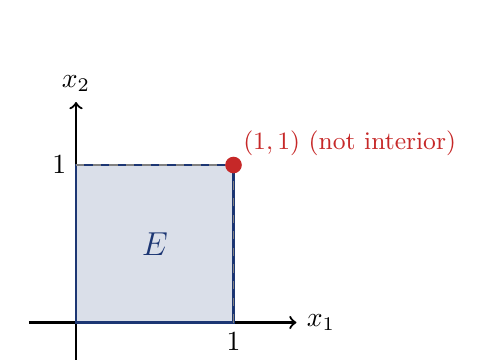
\begin{tikzpicture}[scale=2.0, font=\sffamily]
			% Axes
			\draw[->, thick] (-0.3, 0) -- (1.4, 0) node[right] {$x_1$};
			\draw[->, thick] (0, -0.3) -- (0, 1.4) node[above] {$x_2$};
			
			% Rectangle E = [0,1] \times [0,1] with background fill and shading
			\draw[thick, primaryColor, fill=boxBg] (0, 0) rectangle (1, 1);
			\fill[primaryColor, opacity=0.12] (0, 0) rectangle (1, 1);
			
			% Dashed lines to axes for coordinates
			\draw[dashed, thin, gray] (1, 0) node[below, text=black] {$1$} -- (1, 1);
			\draw[dashed, thin, gray] (0, 1) node[left, text=black] {$1$} -- (1, 1);
			
			% Set Label
			\node[primaryColor, font=\bfseries\large] at (0.5, 0.5) {$E$};
			
			% Highlight boundary point that is not interior (top-right corner)
			\fill[cautionColor] (1, 1) circle (1.5pt);
			\node[anchor=south west, font=\small, text=cautionColor] at (1, 1) {$(1, 1)$ (not interior)};
		\end{tikzpicture}
		\vspace{0.5em}
	\end{example}
	
	
	\begin{example}In $\mathbb{R}^2$, consider the following sets:
		\begin{enumerate}[label=(\alph*)]
			\item $G = \{ (x,y) \in \R^2 : x>0, y>0, x+y<1 \}$
			\item $G = \{ (x,y) \in \R^2 : x>0, y>0, xy<1 \}$
		\end{enumerate}
		Those sets satisfy the interior point condition, and hence they are open sets. The following figures illustrate these sets in the Cartesian plane.
		\vspace{0.5em}
		\begin{center}
			\begin{minipage}[t]{0.48\textwidth}
				\centering
				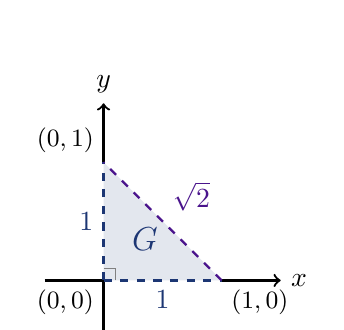
\begin{tikzpicture}[scale=1.5, font=\sffamily]
					% Axes
					\draw[->, thick] (1, 0) -- (1.5, 0) node[right] {$x$};
					\draw[->, thick] (0, 1) -- (0, 1.5) node[above] {$y$};
					\draw[thick] (-0.5,0) -- (0,0);
					\draw[thick] (0,-0.5) -- (0,0);
					% Coordinates of the vertices
					\coordinate (A) at (0, 0); 
					\coordinate (B) at (1, 0); 
					\coordinate (C) at (0, 1); 
					
					% Fill triangle with background color
					\fill[primaryColor, opacity=0.12] (A) -- (B) -- (C) -- cycle;
					
					% Triangle edges
					\draw[thick, primaryColor, dashed] (A) -- (B) node[midway, below] {$1$};
					\draw[thick, primaryColor, dashed] (A) -- (C) node[midway, left] {$1$};
					\draw[thick, theoremColor, dashed] (B) -- (C) node[midway, above right] {$\sqrt{2}$};
					
					% Right angle symbol at origin
					\draw[thin, gray] (0.1, 0) -- (0.1, 0.1) -- (0, 0.1);
					
					% Vertex coordinate labels
					\node[anchor=north east, font=\small] at (A) {$(0,0)$};
					\node[anchor=north west, font=\small] at (B) {$(1,0)$};
					\node[anchor=south east, font=\small] at (C) {$(0,1)$};
					
					% Label for set G inside the triangle
					\node[primaryColor, font=\bfseries\large] at (0.35, 0.35) {$G$};     
				\end{tikzpicture}
				\vspace{0.3em}
				
				\textbf{Figure (a)}
			\end{minipage}%
			\hfill
			\begin{minipage}[t]{0.48\textwidth}
				\centering
				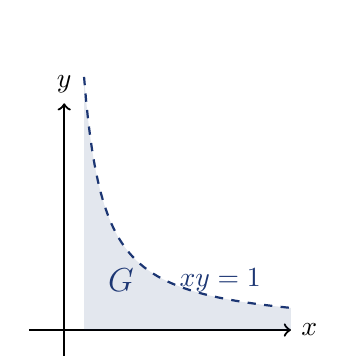
\begin{tikzpicture}[scale=0.9, font=\sffamily]
					% Axes
					\draw[->, thick] (-0.5, 0) -- (3.2, 0) node[right] {$x$};
					\draw[->, thick] (0, -0.5) -- (0, 3.2) node[above] {$y$};
					
					% Shaded region G (x > 0, y > 0, xy < 1 => y < 1/x)
					\fill[primaryColor, opacity=0.12] plot[domain=0.28:3.2, samples=100] (\x, {1/\x}) -- (3.2, 0) -- (0.28, 0) -- cycle;
					
					% The curve xy = 1 bounding the set
					\draw[thick, primaryColor, domain=0.28:3.2, samples=100,dashed] plot (\x, {1/\x});
					\node[text=primaryColor, font=\bfseries] at (2.2, 0.7) {$xy = 1$};
					
					% Label for set G inside the region
					\node[primaryColor, font=\bfseries\large] at (0.8, 0.7) {$G$};
				\end{tikzpicture}
				\vspace{0.3em}
				
				\textbf{Figure (b)}
			\end{minipage}
		\end{center}
	\end{example}
	
	
	\subsection{Properties of Open Sets}
	
	\begin{remark}Basic relationships for interior sets:
		\begin{enumerate}
			\item $(G_1 \cup G_2)^\circ \supseteq G_1^\circ \cup G_2^\circ$
			\item $(G_1 \cap G_2)^\circ = G_1^\circ \cap G_2^\circ$
		\end{enumerate}
	\end{remark}
	
	\begin{theorem}[Properties of Open Sets]
		\begin{enumerate}
			\item $\emptyset$ and $M$ are open sets.
			\item The intersection of any two (finite number of) open sets is open.
			\item The arbitrary union of open sets is open.
		\end{enumerate}
	\end{theorem}
	
	\begin{proof}
		\begin{enumerate}
			\item \textbf{For $\emptyset$ and $M$:} 
			The empty set $\emptyset$ contains no points, so the condition of containing an open ball around every point is vacuously true. For the space $M$ itself, given any point $x \in M$ and any radius $r > 0$, the open ball $B(x; r)$ is a subset of $M$ by definition ($B(x; r) \subseteq M$). Thus, every point in $M$ is an interior point, making $M$ an open set.
			
			\item \textbf{For Finite Intersection:} 
			Let $G_1$ and $G_2$ be two open sets and let $x_0 \in G_1 \cap G_2$. Then $x_0 \in G_1$ and $x_0 \in G_2$. \medskip
			
			\noindent Since $G_1$ and $G_2$ are open, there exist $r_1, r_2 > 0$ such that:
			\[
			B(x_0, r_1) \subseteq G_1 \quad \text{and} \quad B(x_0, r_2) \subseteq G_2
			\]
			Taking $r = \min(r_1, r_2)$, we obtain:
			\[
			B(x_0, r) = B(x_0, r_1) \cap B(x_0, r_2) \subseteq G_1 \cap G_2
			\]
			Therefore, $x_0$ is an interior point of $G_1 \cap G_2$, which proves that $G_1 \cap G_2$ is open.
			
			\vspace{0.5em}
			\begin{center}
				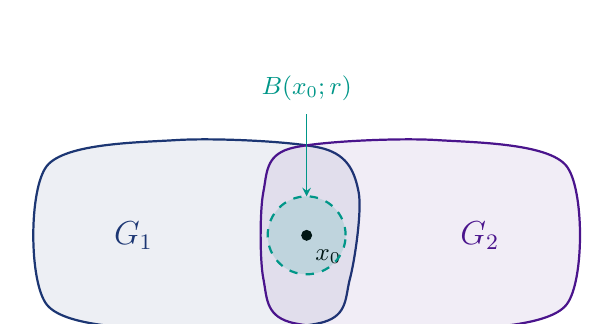
\begin{tikzpicture}[scale=1.1, font=\sffamily]
					% Set G1 (Left horizontal non-regular rectangular shape)
					\draw[thick, primaryColor, fill=primaryColor, fill opacity=0.08, smooth cycle] plot coordinates {
						(-3.0, 0.8) (-1.5, 1.1) (0.2, 1.0) (0.6, 0.5) (0.5, -0.5) (0.2, -1.0) (-1.5, -1.1) (-3.0, -0.8)
					};
					\node[text=primaryColor, font=\bfseries\large] at (-2.0, 0.0) {$G_1$};
					
					% Set G2 (Right horizontal non-regular rectangular shape, overlapping)
					\draw[thick, theoremColor, fill=theoremColor, fill opacity=0.08, smooth cycle] plot coordinates {
						(-0.2, 1.0) (1.5, 1.1) (3.0, 0.8) (3.0, -0.8) (1.5, -1.1) (-0.2, -1.0) (-0.5, -0.5) (-0.5, 0.5)
					};
					\node[text=theoremColor, font=\bfseries\large] at (2.0, 0.0) {$G_2$};
					
					% Point x_0 inside the intersection
					\coordinate (x0) at (0.0, 0.0);
					\fill[black] (x0) circle (1.8pt);
					\node[text=black, font=\small\bfseries] at (0.25, -0.25) {$x_0$};
					
					% Open Ball B(x_0; r) centered at x_0 inside the intersection
					\draw[thick, accentColor, dashed, fill=accentColor, fill opacity=0.15] (x0) circle (0.45cm);
					
					% Label and arrow pointing to the open ball
					\node[text=accentColor, font=\small\bfseries] at (0.0, 1.7) {$B(x_0; r)$};
					\draw[->, >=stealth, thin, accentColor] (0.0, 1.4) -- (0.0, 0.45);
				\end{tikzpicture}
			\end{center}
			\vspace{0.5em}
			
			\item \textbf{For Arbitrary Union:} 
			Let $\{G_i\}_{i \in I}$ be a collection of open sets and let $G = \bigcup_{i \in I} G_i$. If $x \in G$, then there exists an index $k \in I$ such that $x \in G_k$. \medskip
			
			\noindent Since $G_k$ is open, there exists an open ball around $x$ that is contained in $G_k$, and since $G_k \subseteq G$, this ball is also contained in $G$. Thus, every point in $G$ is an interior point, proving that $G$ is open.
		\end{enumerate}
	\end{proof}
	
	
	\lecturetitle{3}{Open Sets, Closed Sets and Accumulation Points}
	
	% =====================================================
	\subsection{Properties of Open Sets}
	
	\begin{takeaway}
		Let $(M,d)$ be a metric space. Then:
		\begin{enumerate}[label=(\arabic*)]
			\item $\emptyset$ and $M$ are open.
			\item A finite intersection of open sets is open.
			\item An arbitrary union of open sets is open.
		\end{enumerate}
	\end{takeaway}
	
	\begin{theorem}
		Any open ball is an open set.
	\end{theorem}
	
	\begin{proof}
		Let $G = B(x_0;R)$ and let $x \in G$. Put
		\[
		r = \tfrac{1}{2}\bigl[R - d(x,x_0)\bigr] > 0 .
		\]
		If $y \in B(x;r)$, then by the triangle inequality
		\[
		d(y,x_0) \le d(y,x) + d(x,x_0) < r + d(x,x_0) < R,
		\]
		so $y \in B(x_0;R)$. Hence $B(x;r) \subseteq G$, so $x$ is an interior point of $G$.
		Since $x \in G$ was arbitrary, $G$ is open.
		
		
	\end{proof}
	
	\noindent Thus, the union of any family of open balls is an open set.
	
	\begin{theorem}
		Any open set can be written as a union of open balls.
	\end{theorem}
	
	\begin{proof}
		Let $G$ be an open set. Then for every $x \in G$ there is $r_x \in \R^+$ such that $B(x;r_x) \subseteq G$. Now,
		\[
		G = \bigcup_{x\in G}\{x\} \subseteq \bigcup_{x\in G} B(x;r_x) \subseteq G .
		\]
		Therefore
		\[
		G = \bigcup_{x\in G} B(x;r_x)
		\]
	\end{proof}
	
	% =====================================================
	\subsection{Closed Sets}
	
	\begin{definition}{Closed Set}
		A set is called \textbf{closed} if its complement is open.
	\end{definition}
	
	\begin{takeaway}
		Main properties of closed sets:
		\begin{enumerate}[label=(\arabic*)]
			\item $M$ and $\emptyset$ are closed.
			\item A finite union of closed sets is closed.
			\item An arbitrary intersection of closed sets is closed.
		\end{enumerate}
	\end{takeaway}
	
	% =====================================================
	\subsection{Accumulation Points of a Set}
	
	\begin{definition}{Accumulation Point}
		A point $x_0 \in M$ is called an \textbf{accumulation point} of a set $E \subseteq M$ if every
		open ball centered at $x_0$ contains a point of $E$ different from $x_0$, that is,
		\[
		\forall r>0 \ \ \exists\, x_1 \in E,\ x_1 \neq x_0,\ \text{ such that } x_1 \in B(x_0;r).
		\]
		Equivalently, $B^*(x_0;r)\cap E \neq \emptyset$ for every $r>0$, where
		$B^*(x_0;r)=B(x_0;r)\setminus\{x_0\}$ is the deleted ball.
	\end{definition}
	
	\begin{example}
		Consider $\R$ (with the usual metric $d(x,y)=|x-y|$). Let
		\[
		E = \Bigl\{1,\tfrac12,\tfrac13,\dots,\tfrac1n,\dots\Bigr\} = \Bigl\{\tfrac1n : n\in\Z^+\Bigr\}.
		\]
		\begin{enumerate}[label=(\arabic*)]
			\item \textbf{$x_0 = 0$ is an accumulation point of $E$.} Let $r\in\R^+$. By the Archimedean
			property there is $n_0\in\Z^+$ with $n_0 > \tfrac1r$, so
			\[
			0 < \tfrac{1}{n_0} < r, \qquad\text{i.e.}\qquad \tfrac{1}{n_0}\in B^*(0;r)\cap E .
			\]
			\item \textbf{This set has no other accumulation points.}
			\begin{enumerate}[label=(\roman*)]
				\item Let $x_0<0$. Take $r=\tfrac12|x_0|$. Then $B(x_0;r)$ contains no point from $E$.
				\item Let $x_0>1$. Take $r=\tfrac12(x_0-1)$. Then $B(x_0;r)\cap E=\emptyset$.
				\item Let $x_0\in E$. Then $x_0=\tfrac{1}{n_0}$ for some $n_0\in\Z^+$. Take
				\[
				r=\tfrac12\Bigl(\tfrac1{n_0}-\tfrac1{n_0+1}\Bigr)=\frac{1}{2n_0(n_0+1)} .
				\]
				Then $B^*(x_0;r)\cap E=\emptyset$.
				\item If $x_0\notin E$ lies between $\tfrac1{n_0+1}$ and $\tfrac1{n_0}$, take
				\[
				r=\tfrac12\min\Bigl\{\tfrac1{n_0}-x_0,\; x_0-\tfrac1{n_0+1}\Bigr\}.
				\]
				Then $B(x_0;r)\cap E=\emptyset$.
			\end{enumerate}
			In each case $x_0$ is not an accumulation point of $E$.
		\end{enumerate}
	\end{example}
	
	\begin{exercise}
		Let
		\[
		E_m=\Bigl\{\tfrac1m+\tfrac1n : n\in\Z^+\Bigr\}, \qquad E=\bigcup_{m=1}^{\infty}E_m .
		\]
		Find the accumulation points of $E$.
	\end{exercise}
	
	\begin{remark}
		The set of accumulation points of a set $E$ is denoted by $E'$.
	\end{remark}
	
	\begin{exercise}[True or false?]
		\label{ex:accum.ofintersectoin}
		\begin{enumerate}[label=(\arabic*)]
			\item $(E_1\cup E_2)' \overset{?}{=} E_1'\cup E_2'$ \quad (\textbf{true})
			\item $(E_1\cap E_2)' \overset{?}{=} E_1'\cap E_2'$ \quad (\textbf{false})
		\end{enumerate}
	\end{exercise}
	
	\begin{example}[Counterexample to Part (2) of Exercise~\ref{ex:accum.ofintersectoin}]
		Let $E_1=\,]0,1[$ and $E_2=\,]1,2[$. Then
		\[
		E_1' = [0,1], \qquad E_2' = [1,2],
		\]
		so $E_1'\cap E_2' = \{1\}$, whereas $E_1\cap E_2=\emptyset$ and hence $(E_1\cap E_2)'=\emptyset$. 
	\end{example}
	
	% =====================================================
	\subsection{Interior and Closure}
	
	\begin{theorem}
		The interior of any set $A$ in a metric space is the largest open set contained in $A$. That is,
		\[
		A^\circ = \bigcup_{\substack{G\subseteq A\\ G\ \text{is open}}} G .
		\]
	\end{theorem}
	
	\begin{proof}
		\textbf{(i)} Let $x_0\in A^\circ$. Then there is an open ball $B(x_0;r)$ such that $B(x_0;r)\subseteq A$. Hence $x_0$ belongs to the right-hand side, so
		\[
		A^\circ \subseteq \bigcup_{\substack{G\subseteq A\\ G\ \text{is open}}} G .
		\]
		
		\textbf{(ii)} Let $x_0\in\bigcup_{G\subseteq A,\ G\text{ open}} G$. Then there exists an open set $G_0\subseteq A$ such that $x_0\in G_0$.
		
		Note that $G_0\subseteq A \Rightarrow G_0^\circ\subseteq A^\circ$. But $G_0^\circ = G_0$ (since $G_0$ is open). Hence $x_0\in G_0\subseteq A^\circ$.
		
	\end{proof}
	
	
	\begin{definition}{Closure}
		The smallest closed set containing $E$ is called the \textbf{closure} of $E$, denoted $\cl{E}$:
		\[
		\cl{E} = \bigcap_{\substack{F\supseteq E\\ F\ \text{is closed}}} F .
		\]
		(This intersection is closed, since an arbitrary intersection of closed sets is closed.)
	\end{definition}
	
	\begin{theorem}
		\label{thm:unionofsetanditsacc.}
		For every set $E$ in a metric space, $\cl{E} = E\cup E'$.
	\end{theorem}
	
	
	
	\begin{exercise}
		Prove the Theorem~\ref{thm:unionofsetanditsacc.}.
	\end{exercise}
	
	\begin{exercise}
		\begin{enumerate}[label=(\arabic*)]
			\item Show that $(E')' \subseteq E'$.
			\item Show that a set is closed if and only if it contains all its accumulation points.
		\end{enumerate}
	\end{exercise}
	
	\begin{exercise}
		Let $E=\,]0,1[$ (with the usual metric of $\R$). Show that
		\[
		E' = [0,1] = \cl{E} \quad\text{and}\quad \boxed{E^\circ = E}.
		\]
	\end{exercise}
	
	
	
	
	
	
	% Lecture 4: start the section counter at 3 so numbering reads 4.1, 4.2, ...
	\setcounter{section}{3}
	\lecturetitle{4}{Sequences in Metric Spaces}
	
	% =====================================================
	\subsection{Sequences and Convergence}
	
	\begin{definition}{Sequence}
		A \textbf{sequence} in a metric space $(M,d)$ is a function from $\Z^+$ to $M$. The terms of such a function can be written as
		\[
		x_1,\, x_2,\, x_3,\, \dots \qquad\text{instead of}\qquad x(1),\, x(2),\, x(3),\, \dots
		\]
		Sometimes we write the whole sequence as $\{x_n\}_{n\in\Z^+}$ or $(x_n)_{n=1}^{\infty}$.
	\end{definition}
	
	\begin{caution}
		The notation $\{x_n : n\in\Z^+\}$ (a set of values) is \textbf{not} a sequence: a set forgets order and
		repetitions. By $\{x_n\}_{n\in\Z^+}$ we always mean the ordered family $(x_n)_{n=1}^\infty$.
	\end{caution}
	\begin{definition}{Convergent Sequence}
		A sequence $\{x_n\}_{n\in\Z^+}$ is called \textbf{convergent} in the space $(M,d)$ if there is an $x_0\in M$ such that
		\[
		\forall\, \varepsilon>0 \ \ \exists\, N_\varepsilon\in\Z^+ \ \text{ s.t. } \ \forall\, n\ge N_\varepsilon \quad d(x_n,x_0)<\varepsilon .
		\]
		In this case we write
		\[
		\lim_{n\to\infty} x_n = x_0 .
		\]
	\end{definition}
	
	\begin{theorem}
		The limit is unique (if it exists).
	\end{theorem}
	
	\begin{proof}
		Suppose that $\lim x_n = x_0$ and $\lim x_n = x_0'$. Then for any $\varepsilon>0$ there exist $N_\varepsilon', N_\varepsilon''\in\Z^+$ such that
		\begin{align*}
			\forall n\ge N_\varepsilon' &\quad d(x_n,x_0) < \varepsilon/2, \\
			\forall n\ge N_\varepsilon'' &\quad d(x_n,x_0') < \varepsilon/2 .
		\end{align*}
		Let $N_\varepsilon=\max\{N_\varepsilon',N_\varepsilon''\}$. Then
		\[
		0 \le d(x_0,x_0') \le d(x_0,x_{N_\varepsilon}) + d(x_{N_\varepsilon},x_0') < \frac{\varepsilon}{2}+\frac{\varepsilon}{2} = \varepsilon .
		\]
		Since $\varepsilon>0$ is arbitrary, $d(x_0,x_0')=0$, hence $x_0=x_0'$.
	\end{proof}
	
	\begin{definition}{Divergent Sequence}
		A sequence which is not convergent is called \textbf{divergent}. That is,
		\[
		\forall\, x_0\in M \ \ \exists\, \varepsilon>0 \ \ \forall\, N_\varepsilon\in\Z^+ \ \ \exists\, n\ge N_\varepsilon \ \text{ s.t. } \ d(x_0,x_n)\ge\varepsilon .
		\]
	\end{definition}
	
	\begin{remark}
		Convergence and divergence depend on the set $M$ and the distance $d$.
	\end{remark}
	
	\begin{example}[Discrete Metric]
		Let $(M,d)$ be a discrete metric space, i.e.\ $d(x,y)=0$ if $x=y$ and $d(x,y)=1$ if $x\neq y$. Then a sequence is convergent if and only if it is eventually constant.
		
		($\Rightarrow$) Suppose $\lim x_n=x_0$ and take $\varepsilon=\tfrac12$. There is $N$ such that
		$d(x_n,x_0)<\tfrac12$ for all $n\ge N$. Since $d$ only takes the values $0$ and $1$,
		this forces $d(x_n,x_0)=0$, i.e.\ $x_n=x_0$ for all $n\ge N$. So $(x_n)$ is eventually constant.
		
		($\Leftarrow$) If $x_n=x_0$ for all $n\ge N$, then $d(x_n,x_0)=0<\varepsilon$ for every $\varepsilon>0$ and all $n\ge N$, so $\lim x_n=x_0$.
	\end{example}
	
	% =====================================================
	\subsection{Cauchy Sequences and Completeness}
	
	\begin{definition}{Cauchy Sequence}
		Let $\{x_n\}_{n\in\Z^+}$ be a sequence in a metric space $(M,d)$. It is called \textbf{Cauchy} if for every $\varepsilon>0$ there is an $N_\varepsilon\in\Z^+$ such that
		\[
		\forall\, m,n\ge N_\varepsilon \quad d(x_n,x_m)<\varepsilon .
		\]
	\end{definition}
	
	\begin{theorem}
		Any convergent sequence is Cauchy.
	\end{theorem}
	
	\begin{proof}
		Suppose that $\lim x_n=x_0$. Then for every $\varepsilon>0$ there is $N_\varepsilon\in\Z^+$ such that
		\begin{align*}
			\forall n\ge N_\varepsilon &\quad d(x_n,x_0)<\varepsilon/2,\\
			\forall m\ge N_\varepsilon &\quad d(x_m,x_0)<\varepsilon/2 .
		\end{align*}
		Hence for $m,n\ge N_\varepsilon$,
		\[
		d(x_m,x_n)\le d(x_m,x_0)+d(x_0,x_n)<\frac{\varepsilon}{2}+\frac{\varepsilon}{2}=\varepsilon .
		\]
	\end{proof}
	
	\begin{definition}{Complete Metric Space}
		A metric space $(M,d)$ is called \textbf{complete} if every Cauchy sequence in $M$ is convergent.
	\end{definition}
	
	\begin{example}
		$\R$ with the usual metric is complete, but $\Q$ with the usual metric is not. Consider the sequence of rational numbers $x_n=\bigl(1+\tfrac1n\bigr)^n$. It converges in $\R$ (to the irrational number $e$), so it is Cauchy. But it has no limit in $\Q$, because limits are unique and $e\notin\Q$.
	\end{example}
	
	% =====================================================
	\subsection{Closure and Completeness of Subsets}
	
	\begin{theorem}
		\label{thm:closure}
		Let $(M,d)$ be a metric space and $A\subseteq M$. Then $x_0\in \cl{A}$ if and only if there is a sequence $\{x_n\}_{n\in\Z^+}\subseteq A$ such that $\lim x_n=x_0$.
	\end{theorem}
	
	\begin{exercise}
		Prove the Theorem~\ref{thm:closure}.
	\end{exercise}
	
	\begin{corollary}
		\label{cor:completemetricandclosness}
		A subset of a complete metric space is complete if and only if it is closed.
	\end{corollary}
	
	\begin{exercise}
		Prove the Corollary~\ref{cor:completemetricandclosness}.
	\end{exercise}
	
	\begin{example}
		$\Z\subseteq\R$ is complete, since it is closed in $\R$ (its complement is a union of open intervals).
		Equivalently, a Cauchy sequence in $\Z$ is eventually constant.
	\end{example}
	
	\begin{example}
		$[a,b]\subseteq\R$ is complete, but $]a,b[$ is not complete if $-\infty<a<b<\infty$ (with the usual metric).
	\end{example}
	
	\begin{exercise}
		Show that
		\[
		(\cl{A})^{c} = (A^{c})^{\circ}.
		\]
	\end{exercise}
	
\end{document}
